\section{Theorie}
\label{sec:Theorie}

\subsection{Grundlagen zu Mikrowellen und Hohlleitern}
\label{subsec:grundlagen}
Mikrowellen sind elektromagnetische Wellen im Frequenzbereich von \SI{300}{\mega\Hz}
bis \SI{300}{\giga\Hz}. Daher sind sie sehr gut für Hohlleiter, da diese in einem
Frequenzbereich von \SI{1}{\giga\Hz} bis \SI{200}{\giga\Hz} arbeiten. Ein Hohlleiter ist
ein Metallrohr, durch das elektromagnetische Wellen verlustarm geleitet werden können.
Sehr gängig sind dabei Rechteckhohlleiter, auf die auch im Folgenden weiter eingegangen
werden soll.

Jeder Hohlleiter kann verschiedene Typen von Wellen, auch Moden genannt, leiten.
Die Moden unterscheiden sich in der Verteilung des elektrischen und des magnetischen
Feldes. Man unterscheidet TE-Moden, bei denen das eletkrische Feld transversal zur
Ausbreitungsrichtung der Welle und TM-Moden, bei denen das magnetische Feld transversal
zur Ausbreitungsrichtung schwingt. Ein spezialfall sind TEM-Moden, bei denen sowohl
das elektrische alsauch das magnetische Feld transversal zur Ausbreitungsrichtung
schwingt. Für jede Mode im Hohlleiter gibt es eine untere Grenzfrequenz, unterhalb
der kein Energietransport im Hohlleiter möglich ist. Sie kommt durch die Abmessungen
des Hohlleiters und die damit verbundenen Randbedingungen zustande.

Im freien Raum gilt der Zusammenhang
\begin{equation}
  c= \lambda_0 f\,.
  \label{eqn:frequenz}
\end{equation}
Dabei ist $c$ die Lichtgeschwindigkeit im Vakuum, $\lambda_0$ die Wellenlänge im
freien Raum und $f$ die Frequenz der Welle.
Für TE- und TM-Moden in einem lufgefüllten Hohlleiter gilt
\begin{align}
  \lambda_{\symup{g}}=\frac{\lambda_0}{\sqrt{1-\left(\frac{\lambda_0}
  {\lambda_{\symup{c}}}\right)^2}} \,, \\
  \lambda_{\symup{c}}=\frac{2}{\sqrt{\left(\frac{m}{a}\right)^2+
  \left(\frac{n}{b}\right)^2}} \,.
  \label{eqn:hohlleiter}
\end{align}
Hier ist $\lambda_{\symup{g}}$ die Wellenlänge im Hohlleiter und $\lambda_{\symup{c}}$
die Grenzwellenlänge im Hohlleiter. $a$ und $b$ sind Länge und breite des Hohlleiters.
$m$ und $n$ sind die Zahlen, die die Mode der Welle bestimmen.
Wie an diesen Formeln zu erkennen ist, ist die Wellenlänge im Hohlleiter
größer als die im freien Raum.

Wird im Hohhleiter ein Teil der Welle an einer Störstelle reflektiert, so bildet
sich eine stehende Welle. Es bilden sich also Minima und Maxima der Einhüllenden
aus, wobei zwei Minima bzw. zwei Maxima eine halbe Wellenlänge voneinander entfernt
sind. Für diese Wellen kann ein Stehwellenverhältnis oder auch SWR (Standing Wave
Ratio) berechnet werden. Es gilt
\begin{equation}
  S=\frac{E_{\symup{max}}}{E_{\symup{min}}}=\frac{|E_{\symup{ein}}|+|E_{\symup{refl}}}
  |{E_{\symup{ein}}|-|E_{\symup{refl}}}\,.
\end{equation}


\subsection{Das Refelxklystron}
\label{subsec:klystron}

\begin{figure}
  \centering
  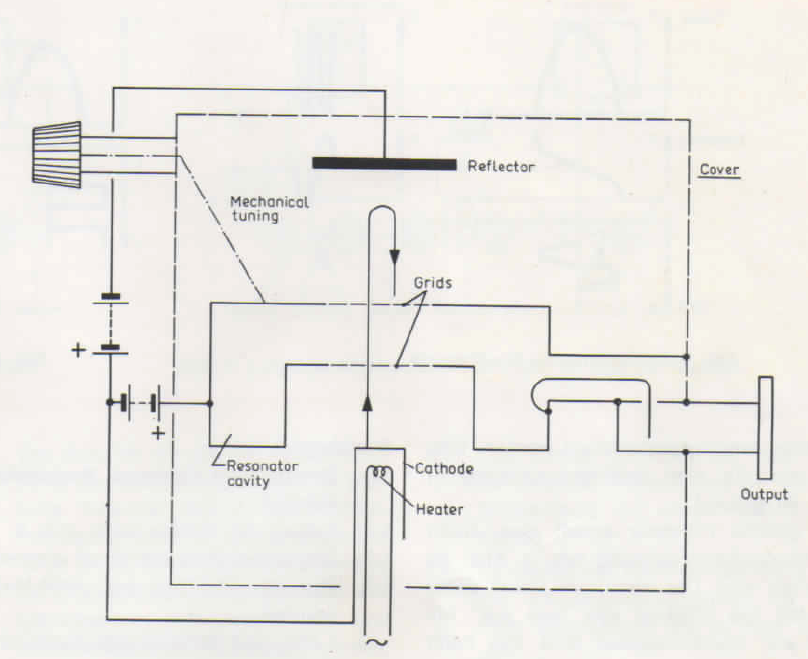
\includegraphics[width=300pt]{data/klystron.png}
  \caption{Skizze der Funktionsweise eines Klystrons \cite{Versuchsanleitung_alt}.}
  \label{fig:klystron}
\end{figure}
